\section{Internal Structure of AES}

\begin{figure}[h] % 'h' means place the figure here if possible
    \centering
    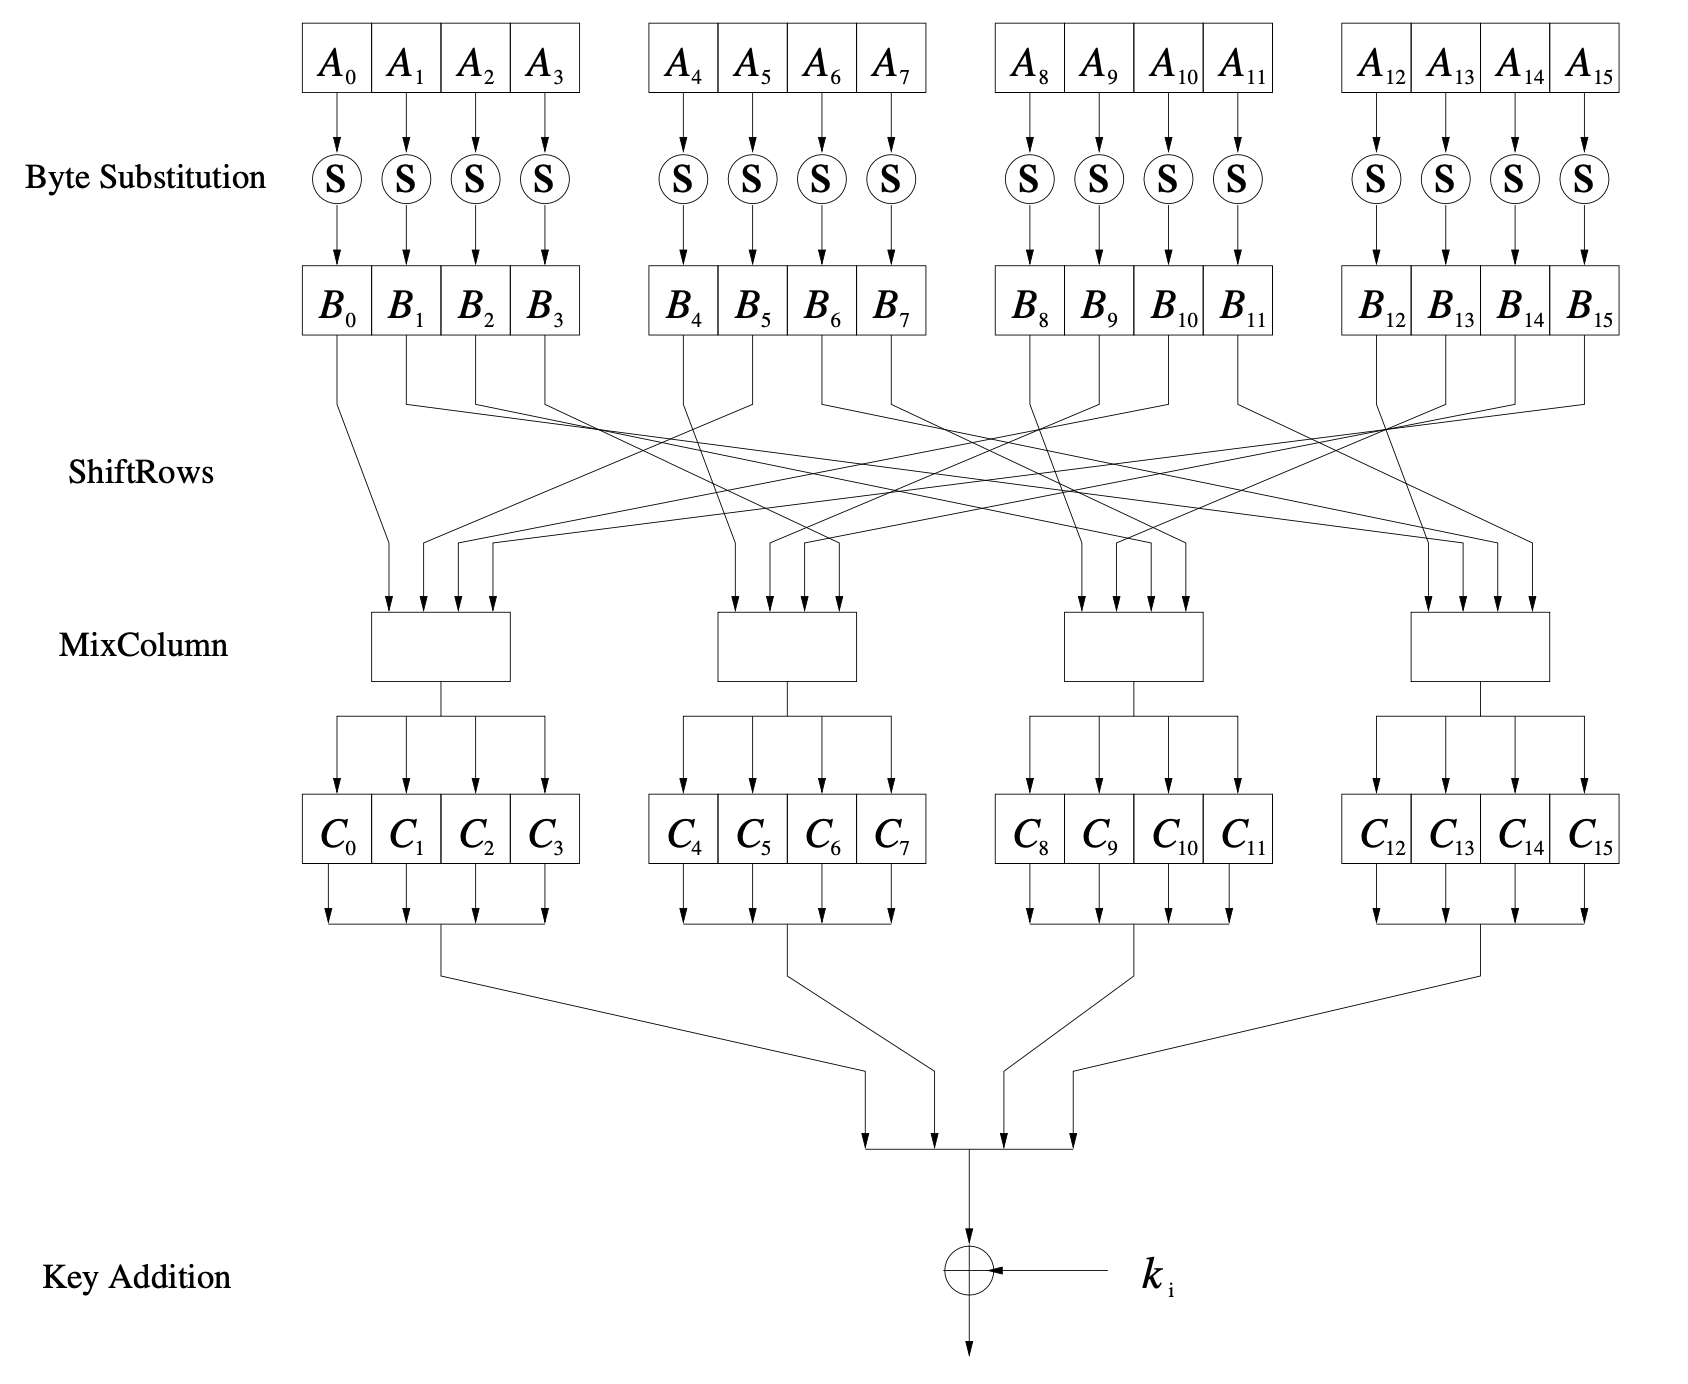
\includegraphics[width=.8\textwidth]{aes-round-function.png} % Adjust width as needed
    \caption{
        AES round function for rounds $1, 2, \dots, n_r-1$.
    }
    \label{fig:aes-round-function} % Reference this figure with \ref{fig:sample_image}
\end{figure}

Figure \ref{fig:aes-round-function} shows the graph of a single AES round. 
The 16-byte input $A_0, \dots, A_{15}$ is fed byte-wise into the S-Box in the Byte Substitution Layer (Section \ref{sec:byte-substitution}).
The 16-byte output $B_0, \dots, B_{15}$ is permutated twice in the \texttt{ShiftRows} layer and mixed by the \texttt{MixColumn} transformation, both in the Diffusion layer (Section \ref{sec:diffusion})
Finally, the 128-bit subkey $k_i$ is XORed with the immediate result in the Key Addition layer (Section \ref{sec:key-addition}).


% \subsection{Byte Substitution Layer}
\label{sec:byte-substitution}



\subsection{Diffusion Layer}
\label{sec:diffusion}

The diffusion spreads the influence of individual bits over the entire state, and spreads the influence of individual bits over the entire state.
The diffusion layer consists of two sublayers: the \texttt{ShiftRows} transformation and the \texttt{MixColumn} transformation.


\subsubsection{\texttt{ShiftRows} Sublayer}

The \texttt{ShiftRows} transformation cyclincally shifts the second row of the state matrix three bytes to the right, the third row by two bytes to the right, and the forth row by one byte to the right.
The first row is not changed.

The purpose of this is to increase the diffusion properties of AES.

% \[
% \begin{align}
%   &\begin{array}{|c|c|}
%     \hline
%     ID & Name \\
%     \hline
%     1 & Alice \\
%     2 & Bob \\
%     \hline
%   \end{array}
%   \quad \longrightarrow \quad
%   \begin{array}{|c|c|}
%     \hline
%     ID & Score \\
%     \hline
%     1 & 85 \\
%     2 & 92 \\
%     \hline
%   \end{array}
% \end{align}
% \]

\begin{equation}
    \begin{array}{c@{\quad \longrightarrow \quad}c}
        \begin{array}{|c|c|c|c|}
        \hline
        B_0 & B_4 & B_8 & B_{12} \\
        \hline
        B_1 & B_5 & B_9 & B_{13} \\
        \hline
        B_2 & B_6 & B_{10} & B_{14} \\
        \hline
        B_3 & B_7 & B_{11} & B_{15} \\
        \hline
        \end{array}
    &
    \begin{array}{|c|c|c|c|}
        \hline
        B_0 & B_4 & B_8 & B_{12} \\
        \hline
        B_5 & B_9 & B_{13} & B_1 \\
        \hline
        B_{10} & B_{14} & B_2 & B_6 \\
        \hline
        B_{15} & B_3 & B_7 & B_{11} \\
        \hline
        \end{array}
    \end{array}
\end{equation}





\subsubsection{\texttt{MixColumn} Sublayer}

The \texttt{MixColumn} transformation is a linear transformation which mixes each column of the state matrix. 
\begin{align}
    MixColumn(B) &= C\\
    \begin{pmatrix}
        02 & 03 & 01 & 01\\
        01 & 02 & 03 & 01\\
        01 & 01 & 02 & 03\\
        03 & 01 & 01 & 02
    \end{pmatrix}
    \cdot
    \begin{pmatrix}
        B_0 & B_4 & B_8 & B_{12} \\
        B_5 & B_9 & B_{13} & B_1 \\
        B_{10} & B_{14} & B_2 & B_6 \\
        B_{15} & B_3 & B_7 & B_{11} \\
    \end{pmatrix}
    &=
    \begin{pmatrix}
        C_0 & C_4 & C_8 & C_{12} \\
        C_1 & C_5 & C_9 & C_{13} \\
        C_2 & C_6 & C_{10} & C_{14} \\
        C_3 & C_7 & C_{11} & C_{15} \\
    \end{pmatrix}
\end{align}
with $B$ being the 16-byte input state after \texttt{ShiftRows} operation given in Equation \ref{} and C being the 16-byte output state.
Each vector column of B is multiplied by a fixed $4 \times 4$ matrix (containing constant entries).


\subsection{Key Addition Layer}
\label{sec:key-addition}